\chapter{Some implementation details}
\label{cha:implementation}

Software engineering decisions, problems, solutions?, and resignations... :P


----

Why re-implement the calibration estimation package?

Why re-implement the robot\_state\_publisher? Explain the how to Publish the /tf tree?
Why KDL? KDL structures are not modificable, so it was needed to re-create KDL once the urdf is updated.

RViz and Markers! Republish everytime!

% \subsection{}
* Quaternions: used to avoid singularities...

* Data/Views in different order... explain... some views aren't visible for all the cameras.

(optional)
Why Ceres?


\section{Fails and solutions}

Explain why it fails
\begin{figure}[!htbp]
 \centering
 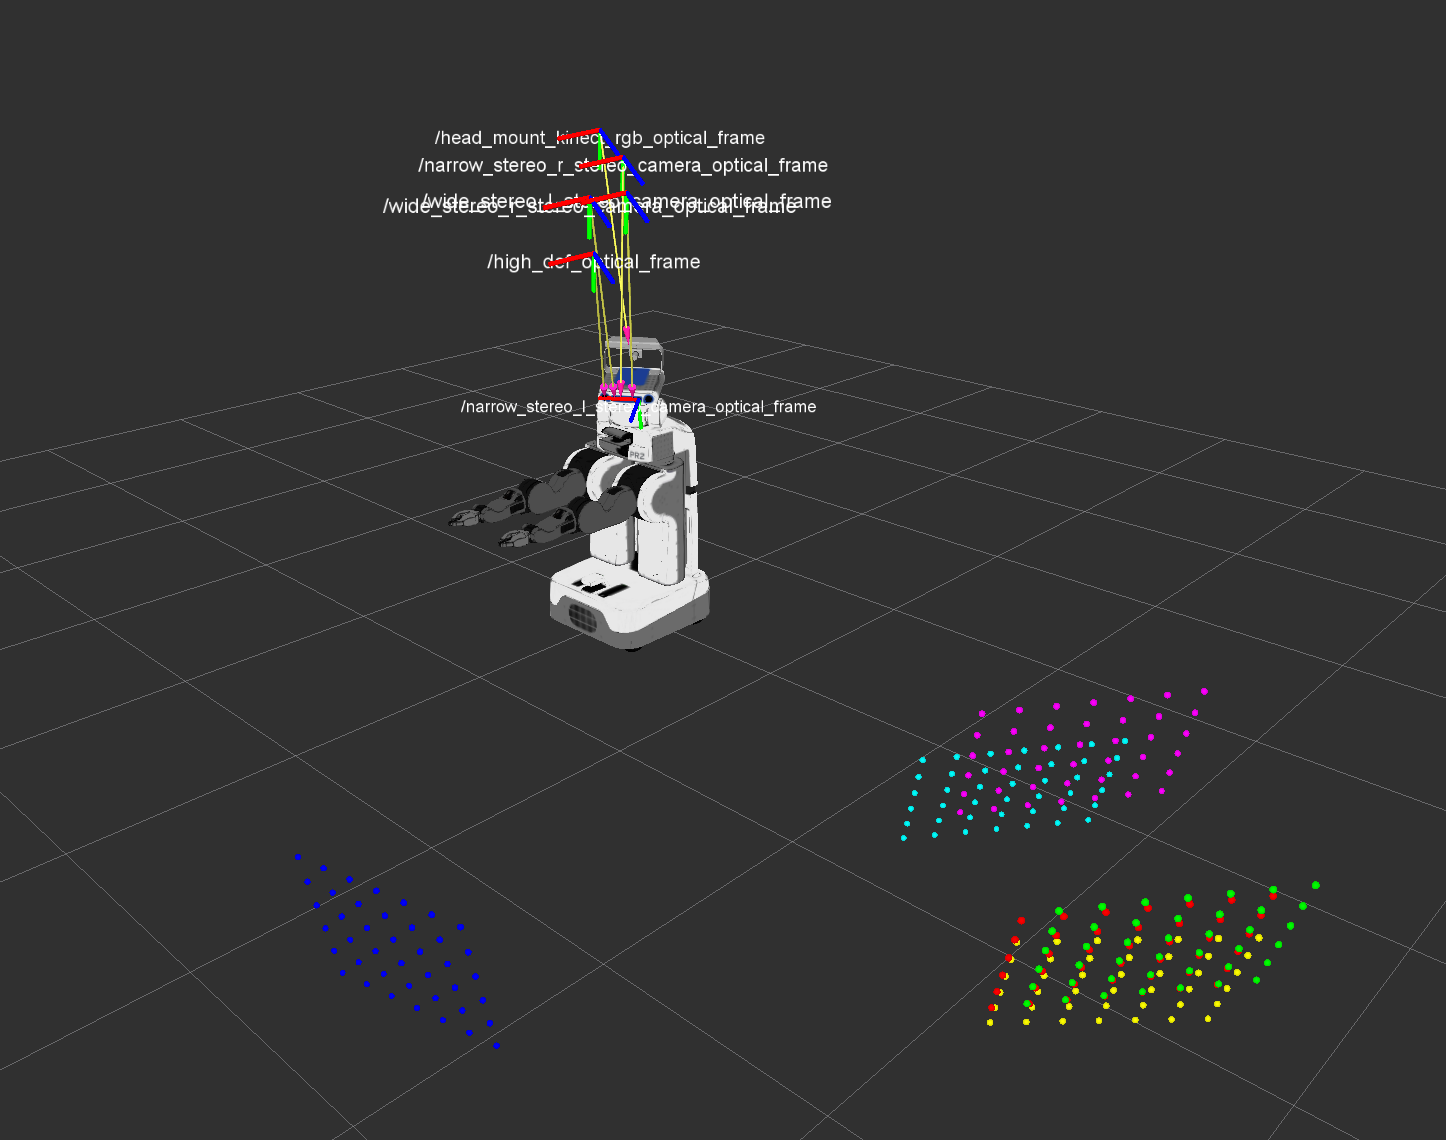
\includegraphics[width=0.5\textwidth]{images/screenshots/optimization_failer02_2.png}
 \caption{Initials versions}
 \label{fig:optimization_failer}
\end{figure}


Triangulation fails... no solution in the moment of writing this thesis :( I couldn't find the bug
\begin{figure}[!htbp]
 \centering
 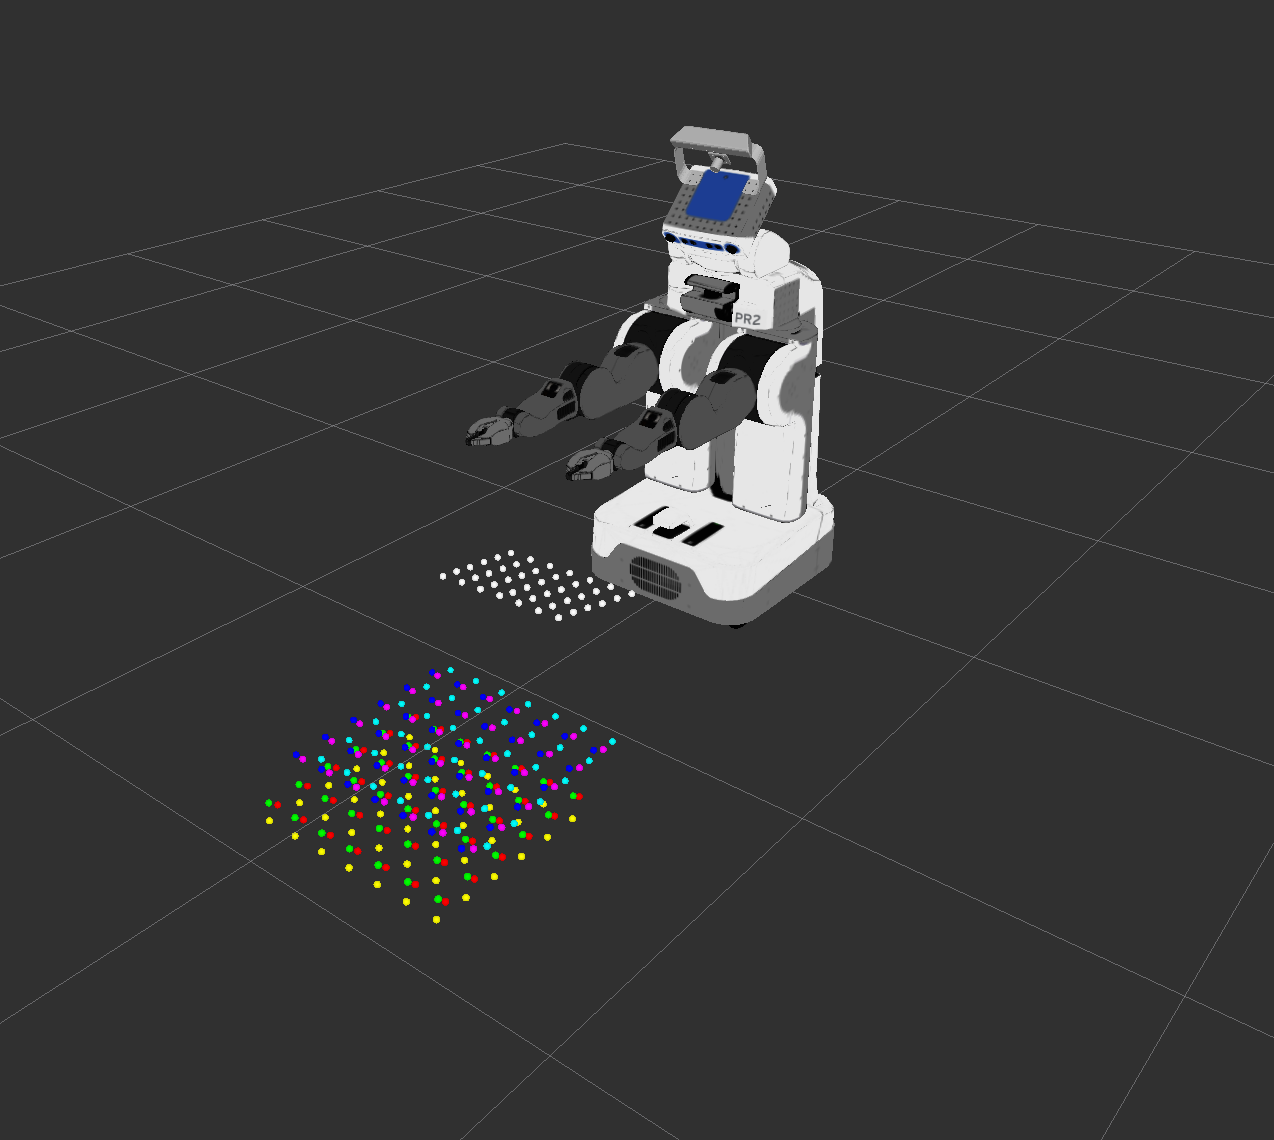
\includegraphics[width=0.5\textwidth]{images/screenshots/triangulation_fails.png}
 \caption{Triangulation fails, white dots}
 \label{fig:triangulation_fails}
\end{figure}




\chapter{Extra work}
\label{cha:extra}

(this chapter is more than optional)

Work not related to the thesis, but time consuming, like commits in Ceres, fixed bugs in URDF dom (export\_urdf() function), etc...



\chapter{Future work}
\label{cha:future}

ideas and all the things I didn't finish but I supposed to... :P
